% Materialer og metoder 2/5
%I dette kapitlet skal du skrive om hvordan du har gått frem metodisk, og vise hvordan valg av design og metode egner seg til å svare på problemstillingen din.

%Kapitlet må kunne gi svar på disse spørsmålene:

%Hvordan samlet du inn datamaterialet?
%Hvordan behandlet du dataene du samlet inn?
%Hvorfor valgte du disse metodene?
%Hva er styrkene og svakehetene ved disse metodene?
%Du skal også si noe om hvorfor du har gjort din undersøkelse på den måten du gjorde – og da peke på styrker og svakheter. I tillegg skal du drøfte etiske aspekter ved prosjektet. På den måten viser du at du har kommet frem til resultatene på en pålitelig og troverdig måte, men også at du er reflektert og kritisk overfor arbeidet du har gjort.

%Husk også at du her, slik som i teorikapitlet, bare skal skrive om det metodiske som er relevant for din studie.
\section{Material og metode}
\label{part:method}

%Dette kapitlet er obligatorisk for alle forsøksoppgaver. Det bør innledes med et flytskjema/oversikt og en beskrivelse som letter leserens forståelse av hva som er gjort. Dette gjelder både for rene analyseoppgaver og for produktutviklingsoppgaver. 

%Beskrivelsen av materialer og metoder skal være tilstrekkelig detaljert slik at andre kan vurdere arbeidet og om ønskelig gjenta forsøkene. Samtidig må man unngå å fylle opp rapporten med unødige detaljer. Dersom det er brukt en velkjent metode, er det nok å bruke metodens offisielle navn og henvise til offisiell kilde. Hvis det var nødvendig med modifikasjoner eller andre tilpasninger i forhold til metoden, må dette beskrives. Eventuell teori om metoden, hører hjemme i teoridelen. Beskriv det dere har gjort og ikke det dere skulle ha gjort. 

%Hensikten med kapitlet Materialer og metoder er at andre skal kunne utføre det samme arbeidet på samme måte. Da må alle nødvendige opplysninger være med.

Trening av kunstige nevrale nettverk gjøres i seks steg. Det ble trent opp to modeller, en RetinaNet-modell og en YOLOv4-modell. RetinaNet hadde forhåndstrente vekter fra en modell trent på COCO-datasettet til Microsoft \cite{Lin m.fl. 2015 s. 1}. YOLOv4 hadde forhåndstrente vekter fra en «Darknet-modell», modellene ble ikke trent fra scratch. %You should design a model which achieves 85 \% validation accuracy on the given dataset.

Microsoft Azure-plattformen ble anvendt til å trene modellene. Microsoft tilbyr Nvidia Titan GPU-er i skyen. Å anvende GPU-er når en trener kunstige nevrale nettverk gjør at treningen tar mindre tid \cite{Dean m.fl. 2012 s. 1}.

Kildekoden kan lastes ned fra GitHub.\footnote{\url{https://github.com/alanhaugen/TMAT3004-Bacheloroppgave}}

\subsection{Å forstå problemet}

Mengden av to fiskeslag, torsk og sei, skulle telles med maskinsyn. Det er to klasser. Bilder av hver fisk med korrekt label-data ble samlet og modellene RetinaNet og YOLOv4 ble valgt, de er store nettverk som kan forstå og trenes på bilder.

\subsection{Få tak i data}
\label{part:data}

Datasettet bestod av bilder fra en lagringsmerd av torsk, og bilder av sei fra Havbruksstasjonen i Tromsø. Se figur \ref{fig:data} og \ref{fig:nofima}. Opptakene av fiskene ble laget av Nofima og ble omgjort til bilder. Label-data ble lagt inn manuelt. Se figur \ref{fig:dataset_tool}. Dataen av torsk var fargebilder, så de bestod av tre kanaler, og hadde størrelsen 1920 $\times$ 1080. Bildene av sei var gråtoner, kun en kanal, og hadde størrelsen 640 $\times$ 480. %You need to achieve 85 \% accuracy for validation data to successfully complete this assignment. Check it out here.

\begin{figure}[h!]
\begin{center} 
\includegraphics[scale=0.05]{../data/train/atlantic_cod/fish_2690}
\includegraphics[scale=0.05]{../data/train/atlantic_cod/fish_6040}
\includegraphics[scale=0.05]{../data/train/atlantic_cod/fish_8540}
\includegraphics[scale=0.05]{../data/train/atlantic_cod/fish_10440}
\includegraphics[scale=0.05]{../data/train/atlantic_cod/fish_4940}
\includegraphics[scale=0.05]{../data/train/atlantic_cod/fish_5740}
\caption{\small \sl Figuren viser eksempelbilder fra en video av en lagringsmerd med torsk. Disse bildene er en del av datasettet anvendt for deteksjon av torsk og sei. \cite{Nofima 2020} \label{fig:data}} 
\end{center} 
\end{figure} 

\begin{figure}[h!]
\begin{center} 
\includegraphics[scale=0.05,angle=-90,origin=c]{figures/camera_1}
\includegraphics[scale=0.05,angle=-90,origin=c]{figures/camera_2}
\includegraphics[scale=0.05]{figures/camera_3}
\caption{\small \sl Figuren viser kamerautstyret som ble anvendt til å lage seidataen. Nofima anskaffet et undervannskamera av typen Steinsvik Orbit-3300 som styres via et MB-3000 kontrollpanel. Foto: Nofima. \cite{Lindberg og Evensen 2020} \label{fig:nofima}} 
\end{center} 
\end{figure} 

Datasettet bestod av 208 bilder av torsk, med til sammen 4582 instanser av torsk i bildene. Det var 604 bilder av sei med 5525 instanser av fisken i bildene. Bildene av torsk og sei ble satt i hver sin mappe. De ble splittet etter forholdet 80/20, 80 \% av dataen var for trening, og 20 \% for validering.

\subsubsection{Utforsk og forstå dataen}

Det er viktig å se på dataen før en begynner å trene et nettverk. Det er viktig å se etter bias i bildene. Det er lurt å gå igjennom hvert eneste bilde, og se om det er noe en kan lære. Torsk- og seibildene kunne bli augmentert, de kunne blant annet bli snudd horisontalt. Det gir dobbelt så mye treningsdata. Vær obs på at ikke alle treningssett tillater dette, for eksempel et datasett med lego. Lego har brikker som er speilbilder av hverandre. Da kan ikke bildene bli snudd horisontalt ettersom det vil gjøre at nettverket ikke kan se forskjell på alle brikkene.

Det var to klasser i datasettet, torsk og sei. Se figur \ref{fig:tree} og tabell \ref{tab:classes}.

\begin{figure}[h!]
\Tree[.data [.labels ] [.train [.atlantic\_cod ]
               [.saithe ]]
          [.validation [.atlantic\_cod ]
                [.saithe ]]]
\caption{\small \sl Figuren viser et tre av mappestrukturen til datasettet. \label{fig:tree}} 
\end{figure} 

\begin{table}[h!]
\bigskip
\centering
\caption{Klassenavn og navneenkoding for datasettet}
\label{tab:classes} 
\begin{tabular}[t]{lcc}
\toprule
Klassekode & Klassenavn    & Norsk klassenavn \\
\midrule
0          & atlantic\_cod & torsk            \\
1          & saithe        & sei         \\
\bottomrule	
\end{tabular}
\end{table}

`\texttt{Labels}'-mappen inneholdt bounding box-data for bildene. Det var en eller flere linjer per `\texttt{.txt}'-fil. Hver linje representerer en bounding box. Representasjonen er i formatet (`xmin', `ymin', `xmax', og `ymax'). Se tabell \ref{tab:bbox}.

Filene som ble brukt til trening og validering ble definert i \texttt{data/fish\_train.txt} og \texttt{data/fish\_test.txt}. Se tabell \ref{tab:fish}.

\begin{table}[b]
\bigskip
\centering
\caption{Label-data for bildet \texttt{data/train/atlantic\_cod/fish\_9440.png}, lagt i filen \texttt{data/labels/fish\_9440.txt}}
\label{tab:bbox} 
\begin{tabular}[t]{lcccc}
\toprule
Klassekode    & xmin      & ymin    & xmax     & ymax \\
\midrule
0 & 238 & 643 & 582 & 882 \\
0 & 80   & 858 & 368 & 1071 \\
\bottomrule	
\end{tabular}
\end{table}

\begin{table}[b]
\bigskip
\centering
\caption{Eksempel på filnavn i \texttt{data/fish\_train.txt} og \texttt{data/fish\_test.txt}}
\label{tab:fish} 
\begin{tabular}[t]{c}
\toprule
Filnavn i \texttt{fish\_test.txt} \\
\midrule
validation/atlantic\_cod/fish\_590.png \\
validation/atlantic\_cod/fish\_640.png \\
\vdots \\
\bottomrule	
\end{tabular}
\end{table}

\subsection{Gjør klar dataen}

Da dataen hadde blitt organisert, og label-data nøye konstruert, så ble nettverkene konfigurert og treningen ble satt i gang. Dataen ble matet inn i treningsprogrammet, inn i deep learning-rammeverkene.

Det ble trent opp to nettverk. Det ene, RetinaNet, er en del av Detectron2 fra Facebook. Den ble trent og konfigurert med PyTorch. Den andre modellen var YOLOv4, den trenes med deep learning-rammeverket Darknet. Konfigurasjon gjøres ved å endre på tekstfiler og kommandolinjeparameterene til rammeverket.

\subsection{Lage label-data}

\begin{figure}[h!]
\begin{center} 
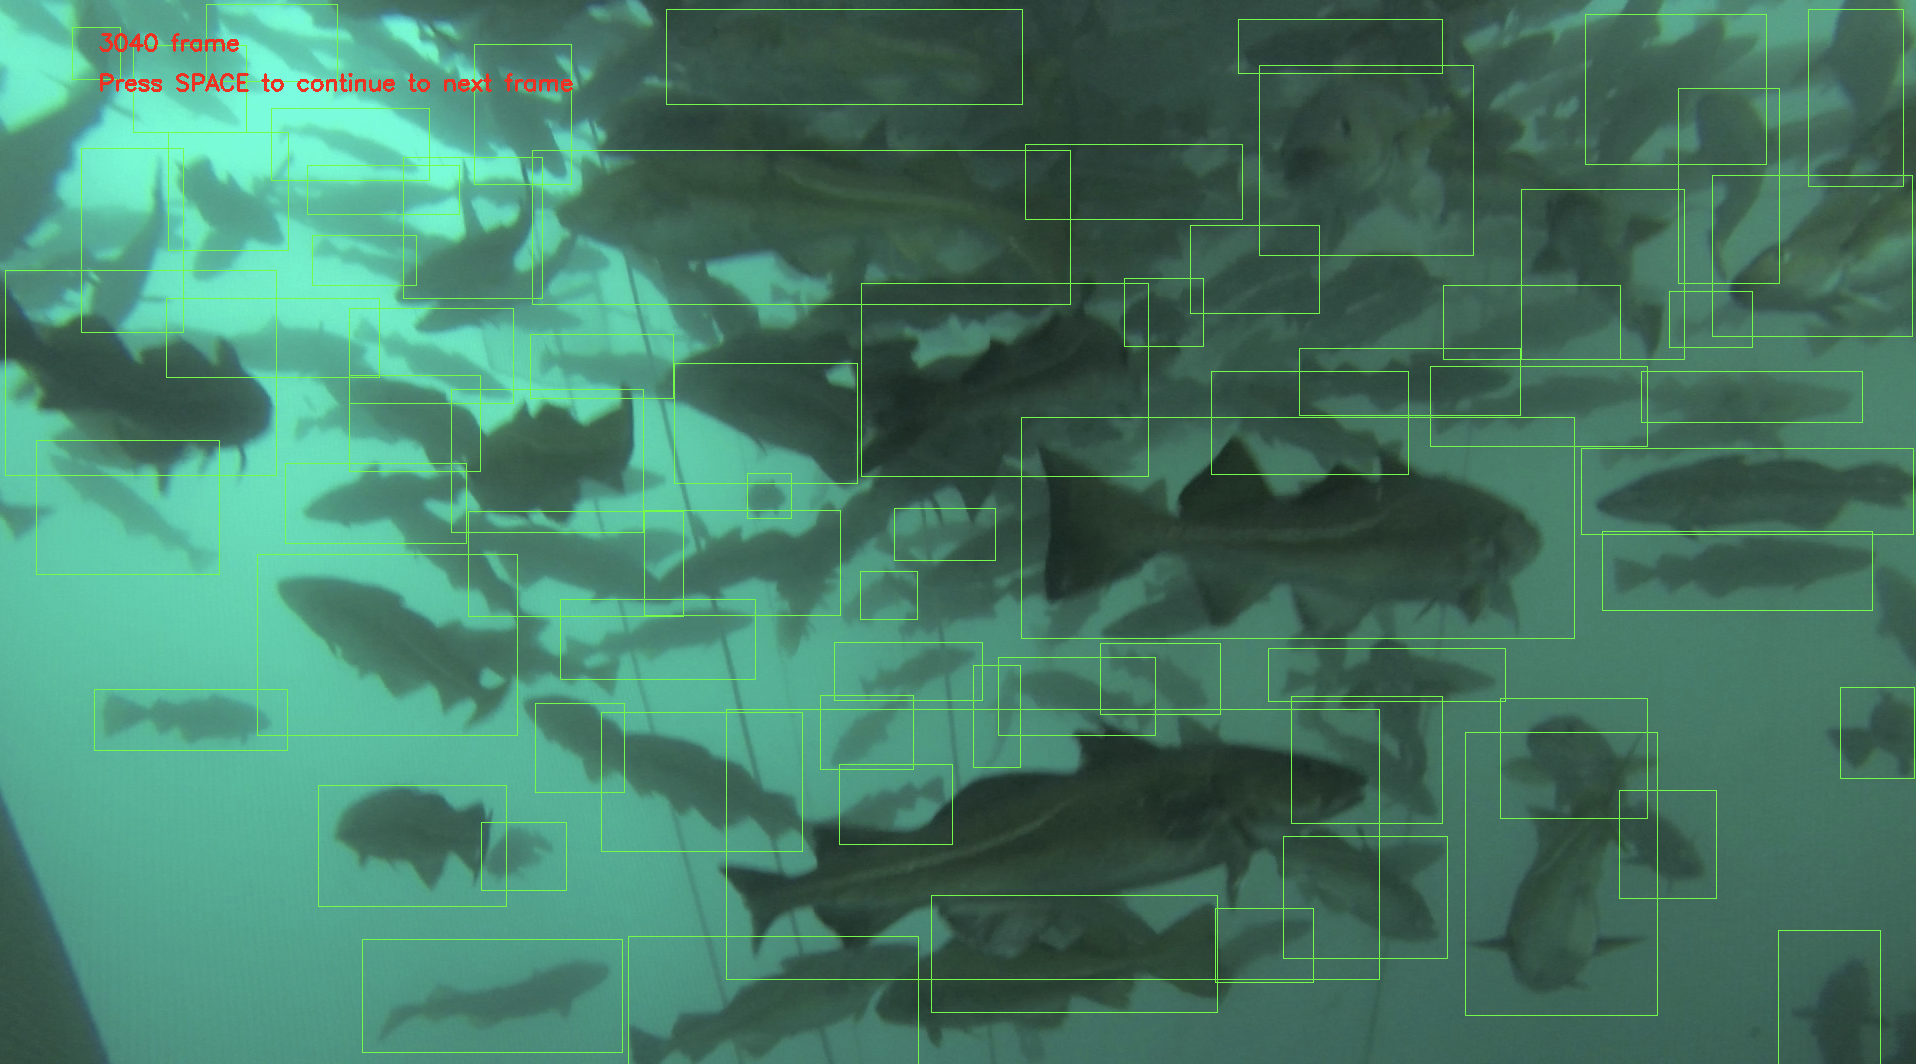
\includegraphics[scale=0.35]{figures/dataset_tool_2}
\caption{\small \sl Et dataprogram som ble utviklet for å lage label-data. Råbildene er basert på opptak fra Nofima \cite{Nofima 2020}. Figuren viser bilde nummer 3040. \label{fig:dataset_tool}} 
\end{center} 
\end{figure} 

Dataprogrammet i figur \ref{fig:dataset_tool} laster inn hvert femtiende bilde fra en video av en lagringsmerd av torsk. Denne videoen er 7 minutter lang. En modell som kan detektere objekter krever å bli trent på bilder av det den skal kjenne igjen, bilder med label-data. Label-data består av klassenummer, og koordinatene `xmin', `ymin', `xmax', og `ymax', som skaper et rektangel rundt objektene som finnes i bildet, for hvert objekt som finnes i treningsdataen. Med dette dataprogrammet så er å lage slik informasjon fra et bilde enkelt, brukeren trenger kun å lage et rektangel rundt hver torsk. Klassenummeret for torsk, her 0, og posisjonene av rektangelet, `xmin', `ymin', `xmax', og `ymax', kjent som objektets ground truth bounding box, lagres til en tekstfil. Rådataen, bilder uten rektanglene eller den røde teksten som er øverst i venstre hjørne, lagres også automatisk til en mappe.

\subsubsection{Dataaugmentering}

Det ble ikke gjort endringer på standardmåten Detectron2 og Darknet gjør dataaugmentering.

\subsubsection{YOLOv4 label-data og bildeformat}

YOLOv4 har et annet label-format sammenlignet med RetinaNet, dessuten krever den bilder i jpeg-formatet, med filutvidelsen `\texttt{.jpg}'. Label-dataen legges sammen med bildene. Konvertering fra RetinaNet sitt format til YOLOv4 ble gjort med et awk-skript. Formatet til YOLOv4 er:

\begin{verbatim}
[klassenavn] [objekt midtpunkt i X] [objekt midtpunkt i Y]
	[objekt vidde i X] [objekt høyde i Y]
\end{verbatim}

Et nyttig verktøy til å konvertere bilder er John Cristy sin Image Magick\footnote{\url{https://imagemagick.org}}. Her er hvordan bildene ble konvertert fra Adobe sitt png-format til jpeg:

\begin{verbatim}
mogrify -format jpg *.png
\end{verbatim}

\subsection{Tren nettverket på et lite utvalg av dataen som en test før en trener et fullt nettverk}

Nettverket ble først trent opp på et utvalg av treningsdataen, for å teste nettverket. 208 bilder med 4582 instanser av torsk ble grunnlaget for de første RetinaNet- og YOLOv4-modellene. Dette steget gjøres som en sanity check før en begynner på trening som kan ta mange timer.

\subsubsection{RetinaNet konfigurasjon og trening}
\label{part:training}

RetinaNet-modellen ble trent med en learning rate på 0,001 over 500 iterasjoner. Modellen brukte vekter fra COCO, den ble lastet ned med Detectron2 fra Detectron2 Model Zoo, den heter COCO-Detection/retinanet\_R\_50\_FPN\_3x.yam. RetinaNet sin score threshold ble satt til 0,5. Batch size var 4.

Et utvalg av programkoden som har blitt skrevet for denne oppgaven har blitt lagt ved i vedlegg \ref{appendix:code}.

Først må bibliotekene lastes inn. Se Python-koden på side \pageref{lst:load} i vedlegg \ref{appendix:code}.

Konfigurasjonen defineres i kodesnutten på side \pageref{lst:config} i vedlegg \ref{appendix:code}.

Konfigurasjonen av batch size, number of iterations og learning rate er de viktigste variablene, det er det neste som settes i listingen under. 

%\begin{lstlisting}[language=Python, caption=Solver konfigurasjon i train.py,label={lst:solver_config}]
\begin{tcolorbox}
\begin{minted}{python}
# batch size
cfg.SOLVER.IMS_PER_BATCH = 4

# choose a good learning rate
cfg.SOLVER.BASE_LR = 0.001

# We need to specify the number of iterations for training
max_iter = 500

cfg.SOLVER.MAX_ITER = max_iter

# number of output class
cfg.MODEL.RETINANET.NUM_CLASSES = len(thing_classes)

# update create ouptput directory
cfg.OUTPUT_DIR = output_dir
os.makedirs(cfg.OUTPUT_DIR, exist_ok=True)
\end{minted}
\end{tcolorbox}
%\end{lstlisting}

Neste kodesnutt er trening, koden finnes også i vedlegg \ref{appendix:code} side \pageref{lst:train}.

%\begin{lstlisting}[language=Python, caption=Treningskode i train.py,label={lst:train}]
\begin{tcolorbox}
\begin{minted}{python}
# Create a trainer instance with the configuration.
trainer = DefaultTrainer(cfg) 

# if rseume=False, because we don't have trained model yet. It
# will download model from model url and load it
trainer.resume_or_load(resume=False)

# start training
trainer.train()
\end{minted}
\end{tcolorbox}
%\end{lstlisting}

%You need to set up the training pipeline with a batchsize of 4 and run the experiment for 100 epochs. Make these changes in the Configrations given below.

\subsubsection{YOLOv4 trening}

Alexey Bochkovskiy sin fork av Darknet ble anvendt, det er en versjon av Joseph Redmon sin Darknet: Open Source Neural Networks in C med Windows- og Linux-støtte. Den støtter nyere versjoner av OpenCV og det som var den nyeste versjonen av YOLO da denne rapporten ble skrevet, YOLOv4, som ble utgitt 23. April 2020 \cite{Bochkovskiy m.fl. 2020}. En god guide til Darknet og YOLO finnes på githuben til Alexey. \cite{Bochkovskiy 2020}

%cuDDN ble installert etter Nvidia sine instrukser. \footnote{\url{https://docs.Nvidia.com/deeplearning/sdk/cudnn-install/index.html#installlinux-tar}}

YOLOv4 ble trent med vekter fra en forhåndstrent modell. Først må darknet installeres. Se under.

\begin{verbatim}
git clone https://github.com/AlexeyAB/darknet
cd darknet
\end{verbatim}

Omgjør linjene GPU=0 og OPENCV=0 til GPU=1 og OPENCV=1 i Makefile.

\begin{lstlisting}[language={}, caption=De første linjene i Makefile]
GPU=1
CUDNN=0
CUDNN_HALF=0
OPENCV=1
AVX=0
OPENMP=0
LIBSO=0
ZED_CAMERA=0 # ZED SDK 3.0 and above
ZED_CAMERA_v2_8=0 # ZED SDK 2.X
\end{lstlisting}

Kompiler rammeverket.

\begin{verbatim}
make
\end{verbatim}

Dette vil kompilere Darknet for GPU-en med OpenCV-støtte.

%For å aktivere GPU-støtte, som vil gjøre treningen mye raskere om en har en Nvidia GPU med nok minne, settes GPU = 1 i Makefile-en, deretter rekompileres rammeverket. Rammeverket rekompileres ved å skrive make clean etterfulgt av make.

For å få gode resultater så ble forhåndstrente vekter for konvolveringslagene lastet ned. Den forhåndstrente darknet modellen tar 162 MiB.

\begin{verbatim}
wget https://github.com/AlexeyAB/darknet/releases/download/\
darknet_yolo_v3_optimal/yolov4.conv.137
cp yolov4.conv.137 build/darknet/x64
\end{verbatim}

Filen obj.data ble laget med følgende innhold.

\begin{lstlisting}[language={}, caption=obj.data]
classes = 1
train  = /yolo/data/fish_train.txt
valid  = /yolo/data/fish_test.txt
names = obj.names
backup = /yolo/backup/
\end{lstlisting}

obj.names ble laget med følgende innhold.

\begin{lstlisting}[language={}, caption=obj.names]
atlantic_cod
saithe
\end{lstlisting}

YOLOv4 må konfigureres.

\begin{verbatim}
cp cfg/yolov4-custom.cfg yolo-obj.cfg
\end{verbatim}

Det er kun en klasse i testutvalget. Følgende endringer ble gjort i yolo-obj.cfg-filen.

\begin{itemize}
  \item linjen batch ble satt til batch=64
  \item linjen subdivisions ble satt til subdivisions=16
  \item linjen max\_batches ble satt til max\_batches = 6000
  \item linjen steps ble satt til steps=4800,5400
  \item størrelsen av nettverket ble satt til width=416 og height=416
  \item linjen classes ble satt til classes=1 for hvert av de tre YOLO-lagene
  \item linjen filters ble satt til filters=18 i hvert av de tre konvolveringslagene, `\texttt{[convolutional]}', som kommer før `\texttt{[yolo]}'
\end{itemize}

For hver linje i \texttt{fish\_train.txt} og \texttt{fish\_test.txt} så ble filendingene omgjort til `\texttt{.jpg}'.

Nettverket ble trent med følgende kommando på Ubuntu Linux-maskinen på Azure.

\begin{verbatim}
./darknet detector train obj.data yolo-obj.cfg yolov4.conv.137 -map
\end{verbatim}

Om en bruker Windows brukes følgende kommando:

\begin{verbatim}
darknet.exe detector train obj.data yolo-obj.cfg yolov4.conv.137 -map
\end{verbatim}

Treningen kan ta flere dager. Etter treningen så ble den beste modellen lastet ned.

\begin{verbatim}
scp awh@public-ip:/yolo/backup/yolo-obj_final.weights yolo.weights
\end{verbatim}

Modellen ble brukt i OpenCV-programmet beskrevet i del \ref{part:opencv}. 

\subsection{Trene modellen på hele datasettet}

Det ble trent opp en ny RetinaNet- og en ny YOLOv4-modell med hele datasettet. Nettverkene hadde blitt testet og fungerte slik som forventet.

Hele datasettet, inkludert seidata, ble lagt til \texttt{fish\_train.txt} og \texttt{fish\_test.txt}. Som tidligere, 80 \% av dataen var treningsdata, 20 \% valideringsdata.

\subsubsection{RetinaNet}

RetinaNet trengte ikke å bli videre konfigurert. Koden som ble skrevet tidligere ble anvendt til å trene nettverket.

\begin{verbatim}
python train.py
\end{verbatim}

\subsubsection{YOLOv4}

YOLOv4 måtte bli konfigurert for to klasser, torsk og sei. Det ble gjort følgende endringer i yolo-obj.cfg-filen.

\begin{itemize}
  \item linjen classes ble satt til classes=2 for hvert av de tre YOLO-lagene
  \item linjen filters ble satt til filters=21 i hver av de tre konvolveringslagene som kommer før YOLO-lagene
\end{itemize}

Linjen classes = 1 ble omgjort til classes = 2 i obj.data. 

Filendingene i \texttt{fish\_train.txt} og \texttt{fish\_test.txt} var `\texttt{.jpg}', som før.

%Learning rate var 0,001, learning rate scheduler ble satt med momentum 0,949 og decay lik 0,0005.
%Optimizers and learning rate schedulers [You can even get good results without a learning rate shceduler]
%Regularization techniques like Data Augmentation, Dropout, BatchNorm

\subsection{Forbedre modellen}

Når modellen har blitt trent ferdig bør den forbedres. Den mest effektive måten å forbedre en deep learning-modell er å endre learning rate i konfigurasjonen, og så trene modellen på nytt. Det kan også hjelpe å bruke en ny modell, vanligvis så er en modell med flere konvolveringslag bedre. Dype nevrale nettverk blir stadig dypere ettersom forskere utvikler nye modeller \cite{Szegedy m.fl. s. 1}. Det er også mulig å trene modellen over flere epoker eller iterasjoner. YOLO-modellen ble oppgradert til YOLOv4. RetinaNet-modellen ble mye bedre når den ble trent over flere iterasjoner. Endringene ble gjort underveis i prosjektet. 

%Lowering learning rate helps
%Adding a convolutional layer helps
%Increasing epochs helps when learning rate is low
%Decreasing batch size ...

\subsection{Inferens}

Inferens er når en trent modell er brukt til å forutsi hva en prøve inneholder. Inferens kalles også for en forward pass. En modell gjør ikke backpropagation når den gjør inferens, backpropagation gjøres for å regne ut nøyaktigheten til modellen og til å oppdatere vektene i modellen, noe som kun skjer under trening. 

\begin{figure}
\begin{center} 
%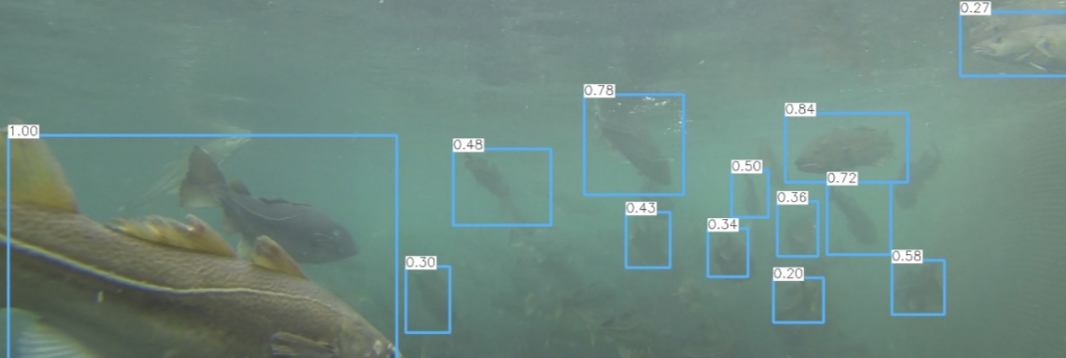
\includegraphics[scale=0.6]{figures/cover}
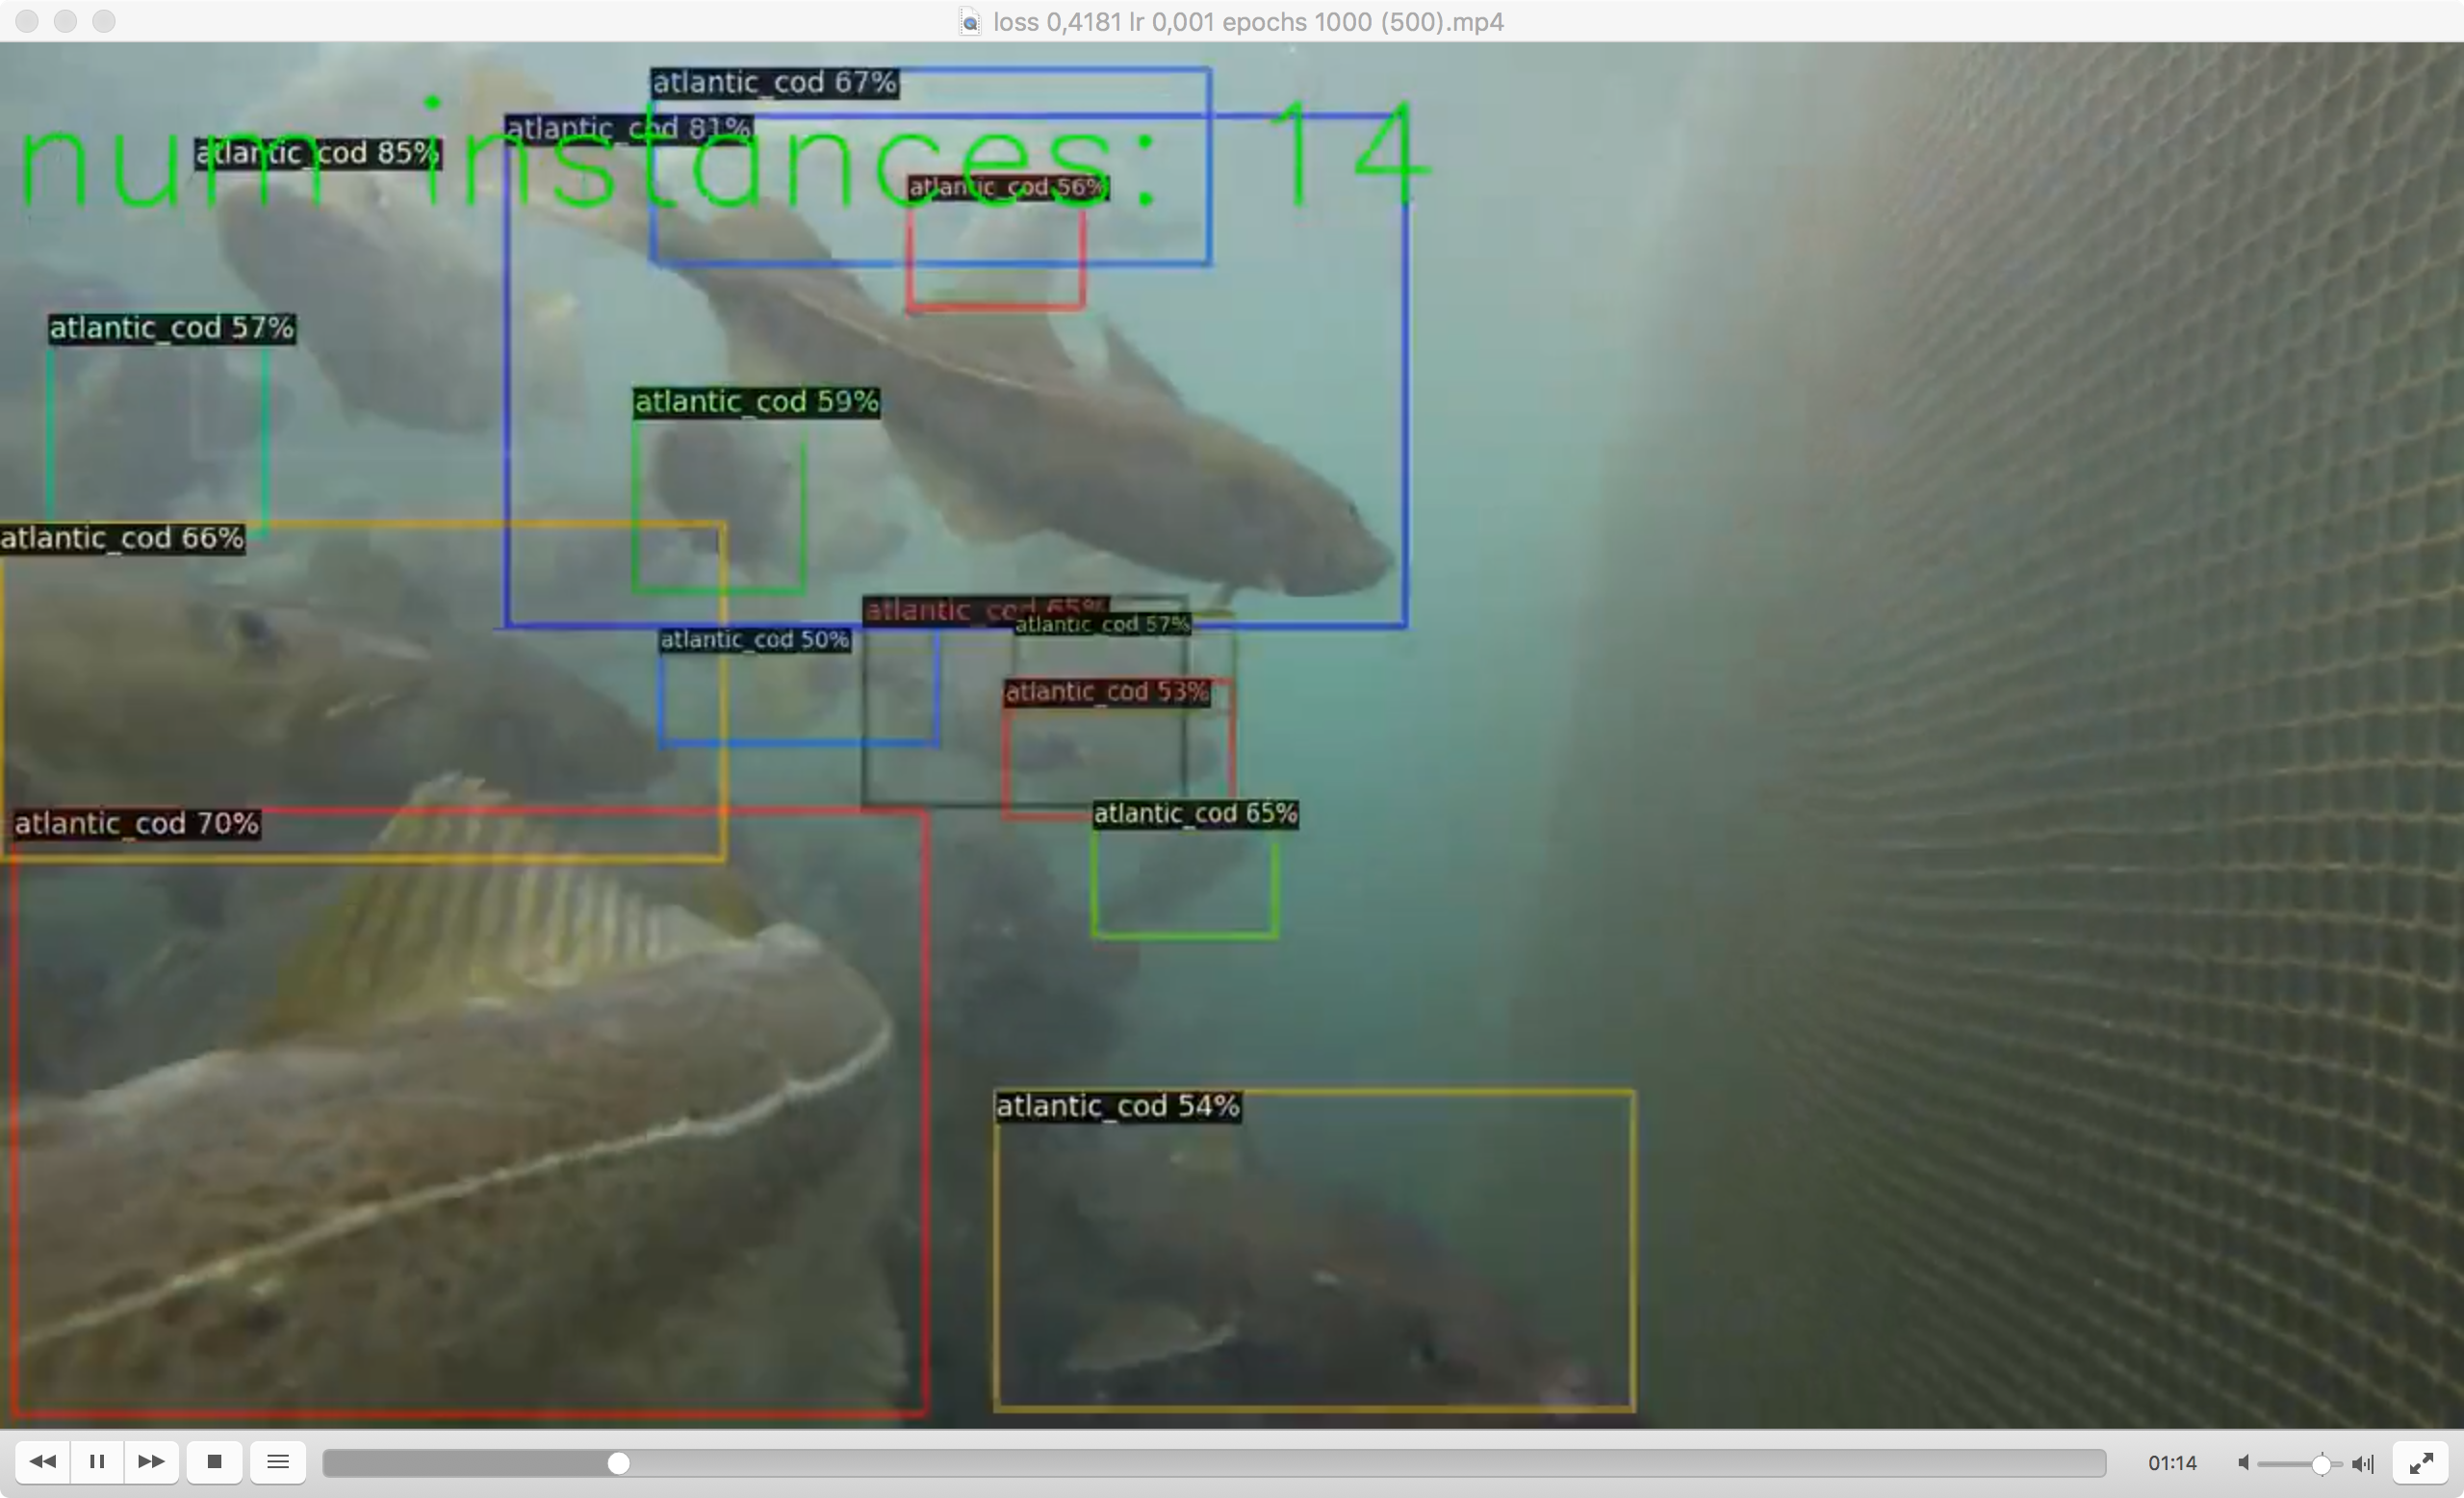
\includegraphics[scale=0.25]{figures/retina-inference-1}
\includegraphics[scale=0.25]{figures/retina-inference-3}
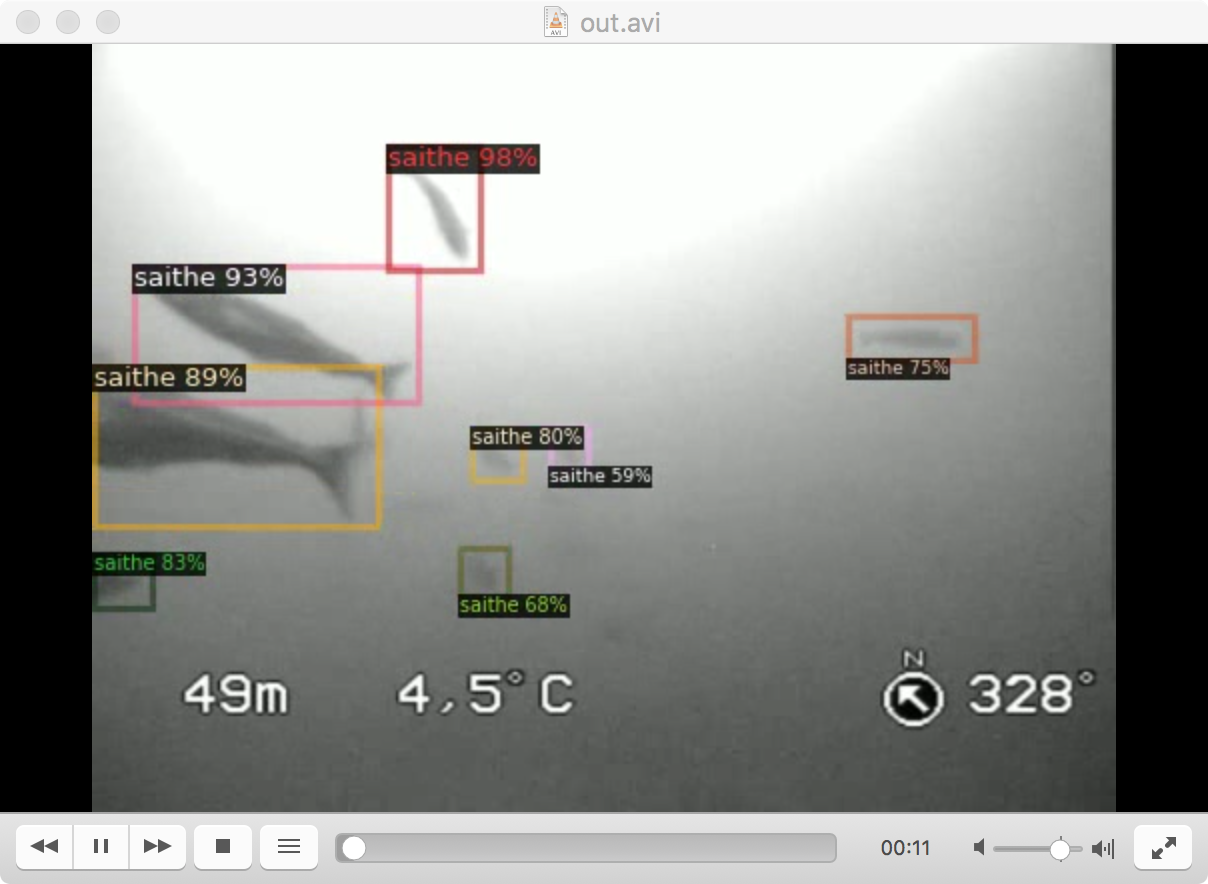
\includegraphics[scale=0.35]{figures/retinanet_inference_saithe}
\caption{\small \sl Inferens med en RetinaNet-model. Råbildene er fra Nofima \cite{Nofima 2020}. \label{fig:inference}} 
\end{center} 
\end{figure} 

\subsubsection{RetinaNet}

Ettersom OpenCV ikke kunne laste inn en PyTorch-modell da denne oppgaven ble skrevet, så ble inferens gjort med Python, og det ble ikke gjort et forsøk på å gjøre inferens i sanntid på en videostrøm med RetinaNet. Se resultater i figur \ref{fig:inference}.

Koden for inferens er i vedlegg A, side \pageref{lst:inferens_retinanet}.

\subsubsection{OpenCV-program} \label{part:opencv}

Det ble skrevet et program i C++ som bruker OpenCV til fiskedeteksjon i sanntid med YOLOv4-modellen. OpenCV hadde fortsatt dårlig støtte av ONIX-formatet, Caffe2-formatet, og PyTorch da denne oppgaven ble skrevet. OpenCV 3.4 ble anvendt, da den nylig fikk støtte for YOLOv4. \cite{Batanina 2020}

\begin{figure}
\begin{center} 
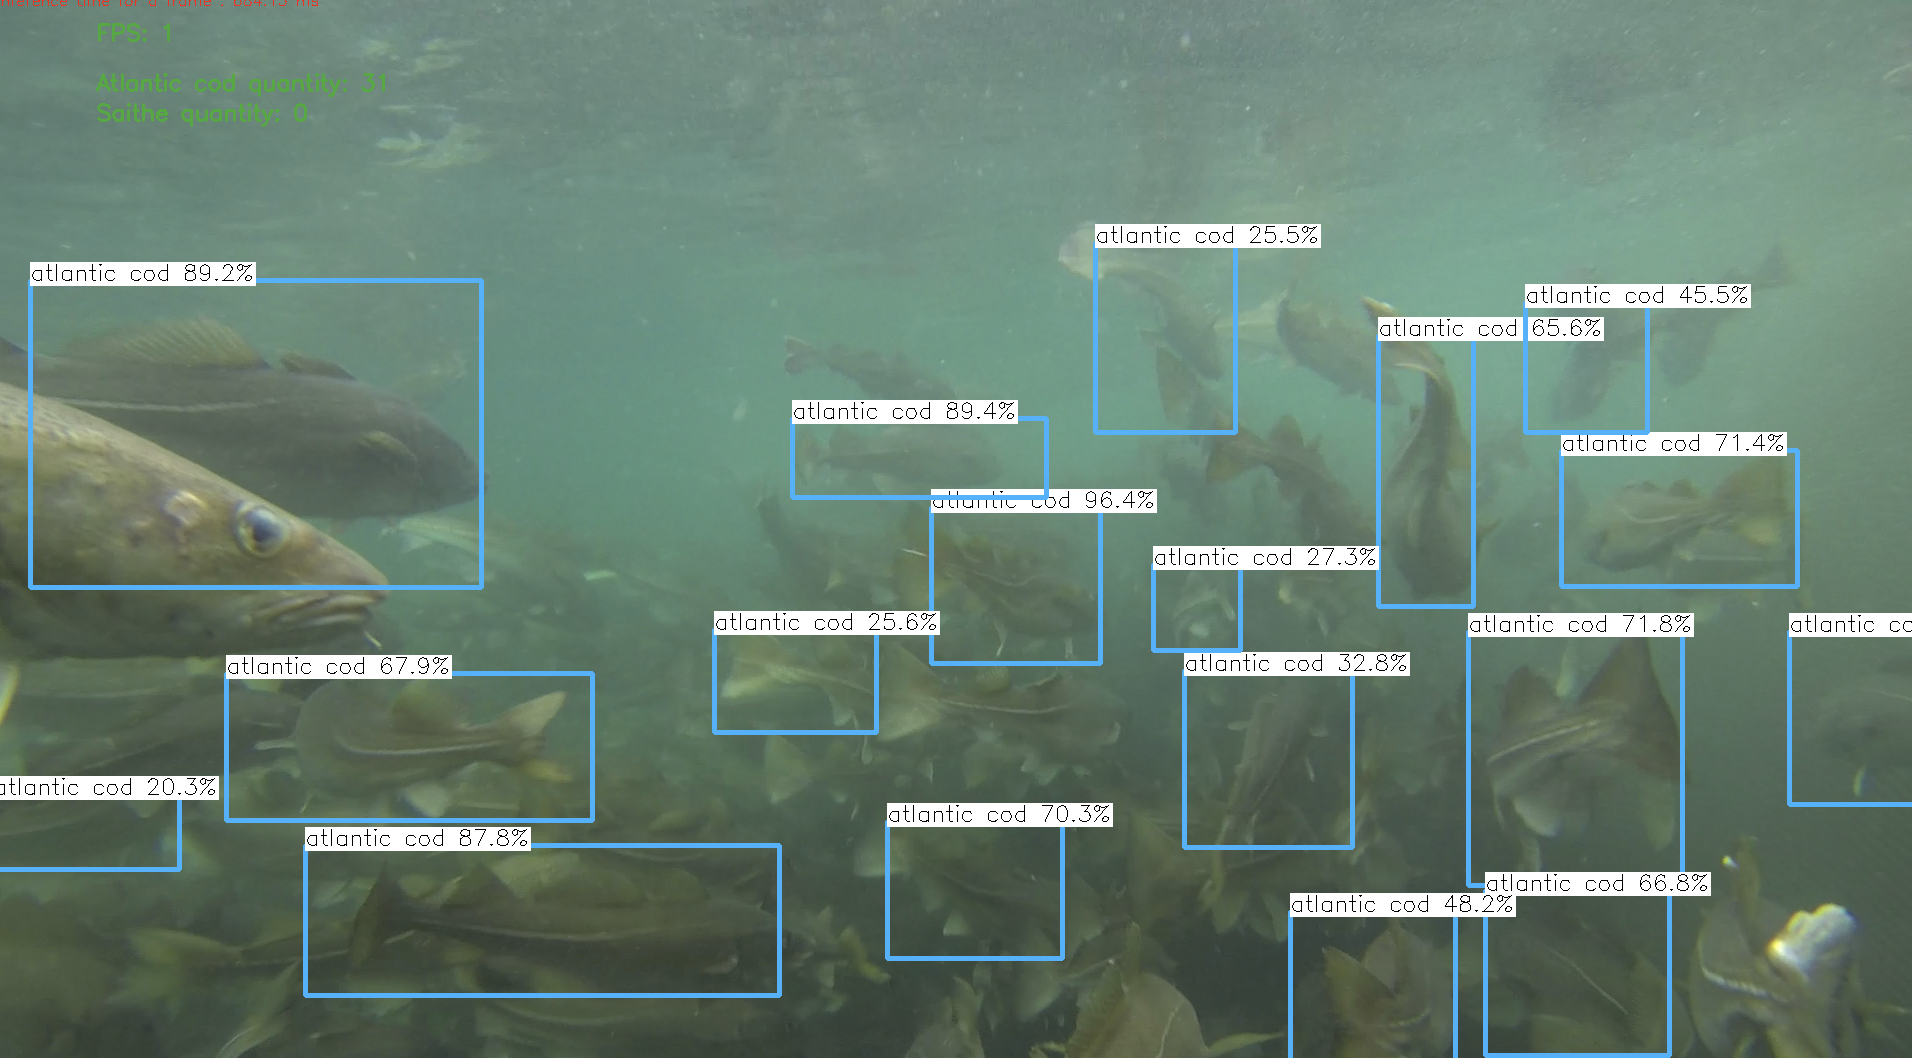
\includegraphics[scale=0.35]{figures/inference_yolo}
\caption{\small \sl Inferens med YOLOv4. Rundt fiskene så lager YOLOv4 bounding boxes der den tror det finnes fisk, og gir den en label basert på det den tror at det er. Her får alle fiskene labelen «atlantic cod», dette er fra en lagringsmerd med torsk. Ved siden av navnet av klassen så står det hvor sikker nettverket er på at den har funnet en torsk, presisjonen av inferensen. I grønn tekst, øverst til venstre, står det at algoritmen kan telle 31 torsk i bildet, og 0 sei. Råbildet er fra Nofima \cite{Lindberg og Evensen 2020}. \label{fig:yolo_inference}} 
\end{center} 
\end{figure} 

Når en lager et program i C++ så må en kompilator og et build-system bli valgt. For Windows så ble msvc++, som er en del av Visual Studio Community 2019, valgt. På macOS så ble clang brukt. Build-systemet cmake ble valgt. Alle disse verktøyene er tilgjengelig gratis, msvc++ er det eneste verktøyet som ikke er et åpen kildekodeprosjekt i tillegg til å være gratis. \texttt{CMakeLists.txt} beskriver programmet. \texttt{CMakelists.txt} er en konfigurasjonsfil for cmake build-systemet, et av build-systemene som kan brukes til å holde styr på C++-programmer. Det er nyttig å ha en IDE, en Integrated Development Environment, når man programmerer i C++. QtCreator open source er et velutviklet IDE som kan laste inn cmake-prosjekter.

OpenCV-prosjektet bruker også cmake, og er også skrevet i C++. Her installeres OpenCV fra kommandolinjen på et Unix-system:

\begin{verbatim}
mkdir opencv-3.4
cd opencv-3.4
git clone https://github.com/opencv/opencv
git clone https://github.com/opencv/opencv_contrib
cd opencv_contrib
git checkout 3.4
cd modules
dir=$(pwd)
cd ../../opencv
git checkout 3.4
mkdir build
cd build
cmake OPENCV_EXTRA_MODULES_PATH=$dir ..
make
make install
\end{verbatim}

\begin{figure}
\begin{center} 
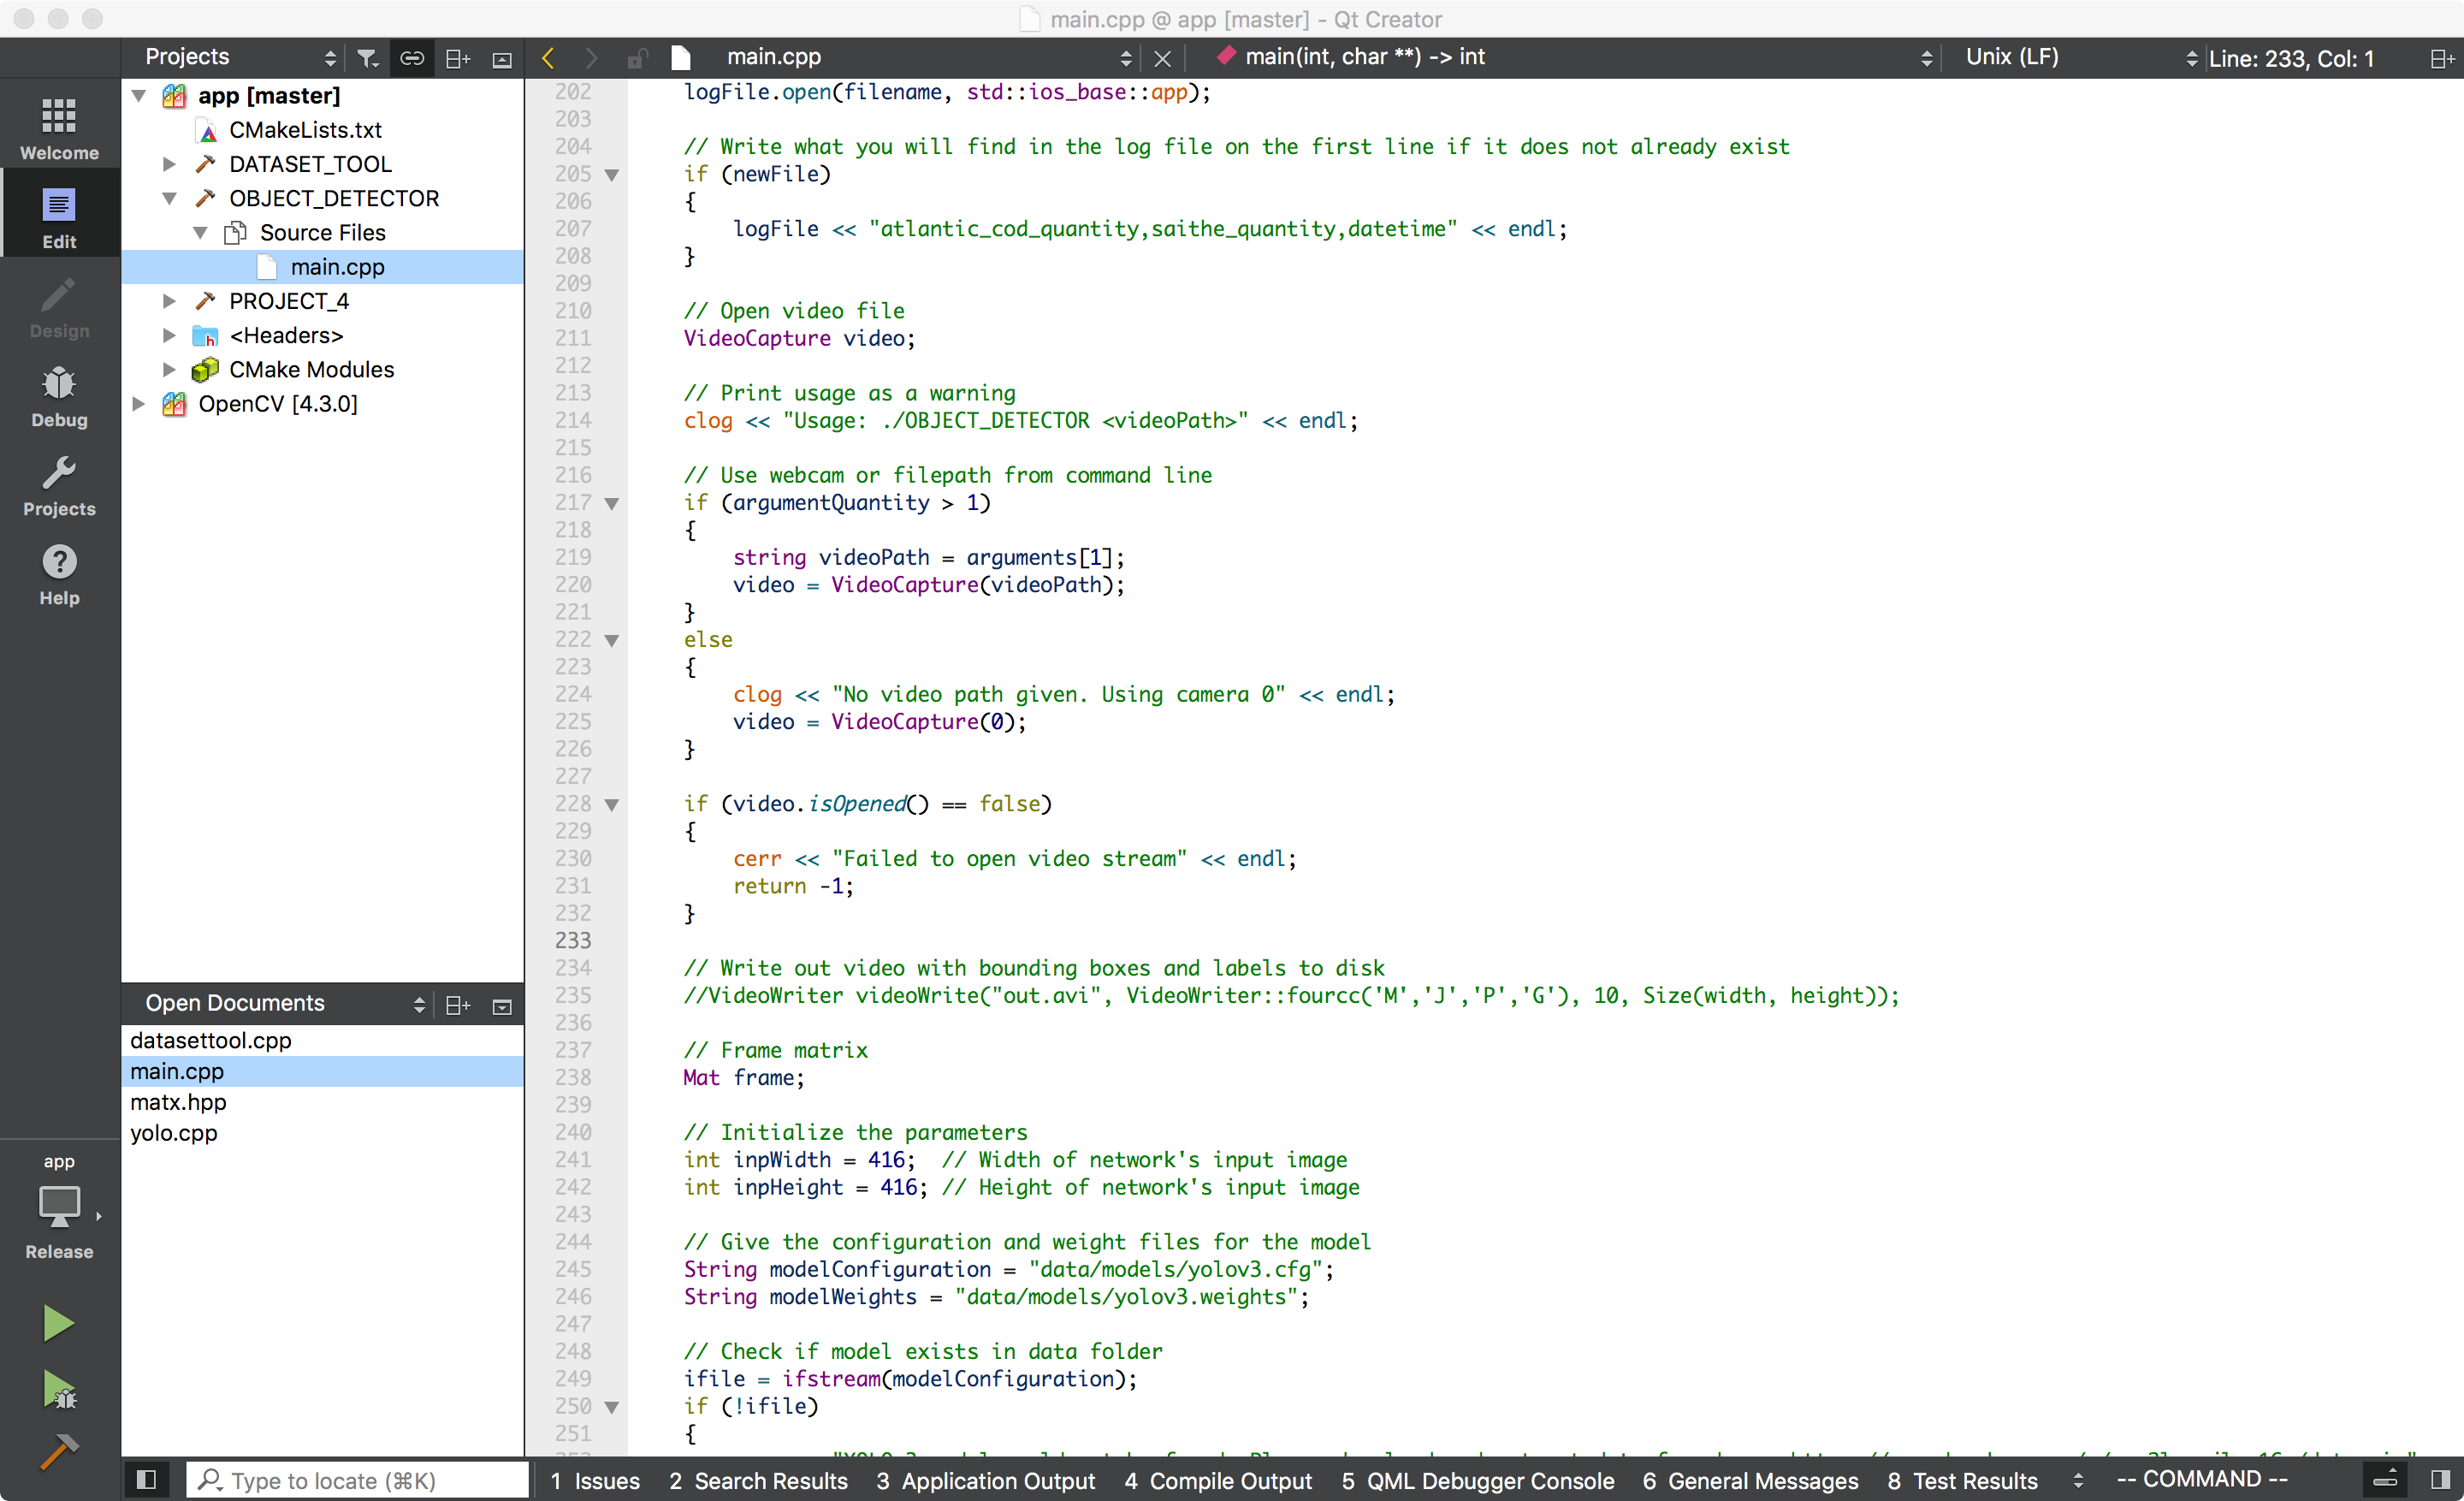
\includegraphics[scale=0.2]{figures/qtcreator}
\caption{\small \sl Figuren viser IDE-et QtCreator med main.cpp hvor OpenCV- og TMAT3004-prosjektene er lastet inn.  \label{fig:qtcreator}} 
\end{center} 
\end{figure} 

Det er også mulig å kompilere OpenCV med hjelp fra QtCreator. QtCreator open source ble lastet ned fra \url{https://www.qt.io/download}. \texttt{CMakeLists.txt} i opencv-3.4/opencv ble åpnet i QtCreator. OPENCV\_EXTRA\_MODULES\_PATH ble satt til opencv\_contrib/modules på filsystemet. Dette kan gjøres fra Projects-modusen i QtCreator. Se sidepanelet i figur \ref{fig:qtcreator}.

Anaconda individual edition med Python 2 ble brukt. Det ble laget en \texttt{CMakeLists.txt}-fil for prosjektet. Se side \pageref{lst:cmake} i vedlegg \ref{appendix:code}. Denne burde muligens endres om andre ønsker å kompilere prosjektet, merk at Anaconda ble installert til hjemmemappen til brukeren. Prosjektet består av to programmer. OBJECT\_DETECTOR gjør fiskedeteksjon. Se figur \ref{fig:yolo_inference}. DATASET\_TOOL ble brukt til å lage label-data ut av videoer. Se figur \ref{fig:dataset_tool}.

OBJECT\_DETECTOR gjør inferens med OpenCV dnn-modulen, den laster inn en YOLOv4-konfigurasjon, en modell, og en videostrøm. Videostrømmen kan komme fra et kamera koblet til maskinen eller en fil på filsystemet. Programmet analyserer videostrømmen og logger mengden torsk og sei som blir observert. Se figur \ref{fig:yolo_inference}.

\texttt{main.cpp} er kildekoden til OBJECT\_DETECTOR. Først lastes bibliotekene inn. Se side \pageref{lst:header} i vedlegg \ref{appendix:code}.

\texttt{getOutputsNames} henter ut label-navn fra det ytterste laget, «the fully connected layer», i modellen. Det er her utmatningene fra modellen er. Se figur \ref{fig:deep} og side \pageref{lst:getOutputsNames} i vedlegg \ref{appendix:code}.

\texttt{drawPred} lager en bounding box rundt objektene som detekteres av modellen. Se side \pageref{lst:drawPred} i vedlegg \ref{appendix:code}.

\texttt{postprocess} henter alle instanser av fiskene i et bilde som er over en non-maxima suppression confidence boundary. Deretter sjekker den om objektet er en torsk eller sei, og teller mengden torsk og sei i bildet. Se side \pageref{lst:postprocess} i vedlegg \ref{appendix:code}.

\texttt{main} er programmets entry point. Det er her dataprogrammet starter. Den åpner en logg, log.csv, og så åpner den en videostrøm. Deretter laster den inn YOLOv4-modellen. Se side \pageref{lst:main} i vedlegg \ref{appendix:code}.

Den siste kodesnutten er programmets main loop. Denne koden repeteres til videoen har gått tom for bilder, eller at brukeren trykker på ESC på tastaturet. For hvert bilde i videostrømmen så lagres antall torsk og sei observert og tidskode til log.csv, med mindre det er ingen torsk eller sei som blir oppdaget. Se side \pageref{lst:mainloop} i vedlegg \ref{appendix:code}.

%\subsection{COCO Detection Evaluation} % For analyse kapittelet?

\subsection{Segmentering}

Det ble laget label-data for segmentering i datapgrogrammet labelme \cite{Wada 2016}. Se figur \ref{fig:labelme}. Det ble ikke gjort et forsøk på segmentering da objektdeteksjon ga bedre resultater enn forventet.

\begin{figure}[h!]
\begin{center} 
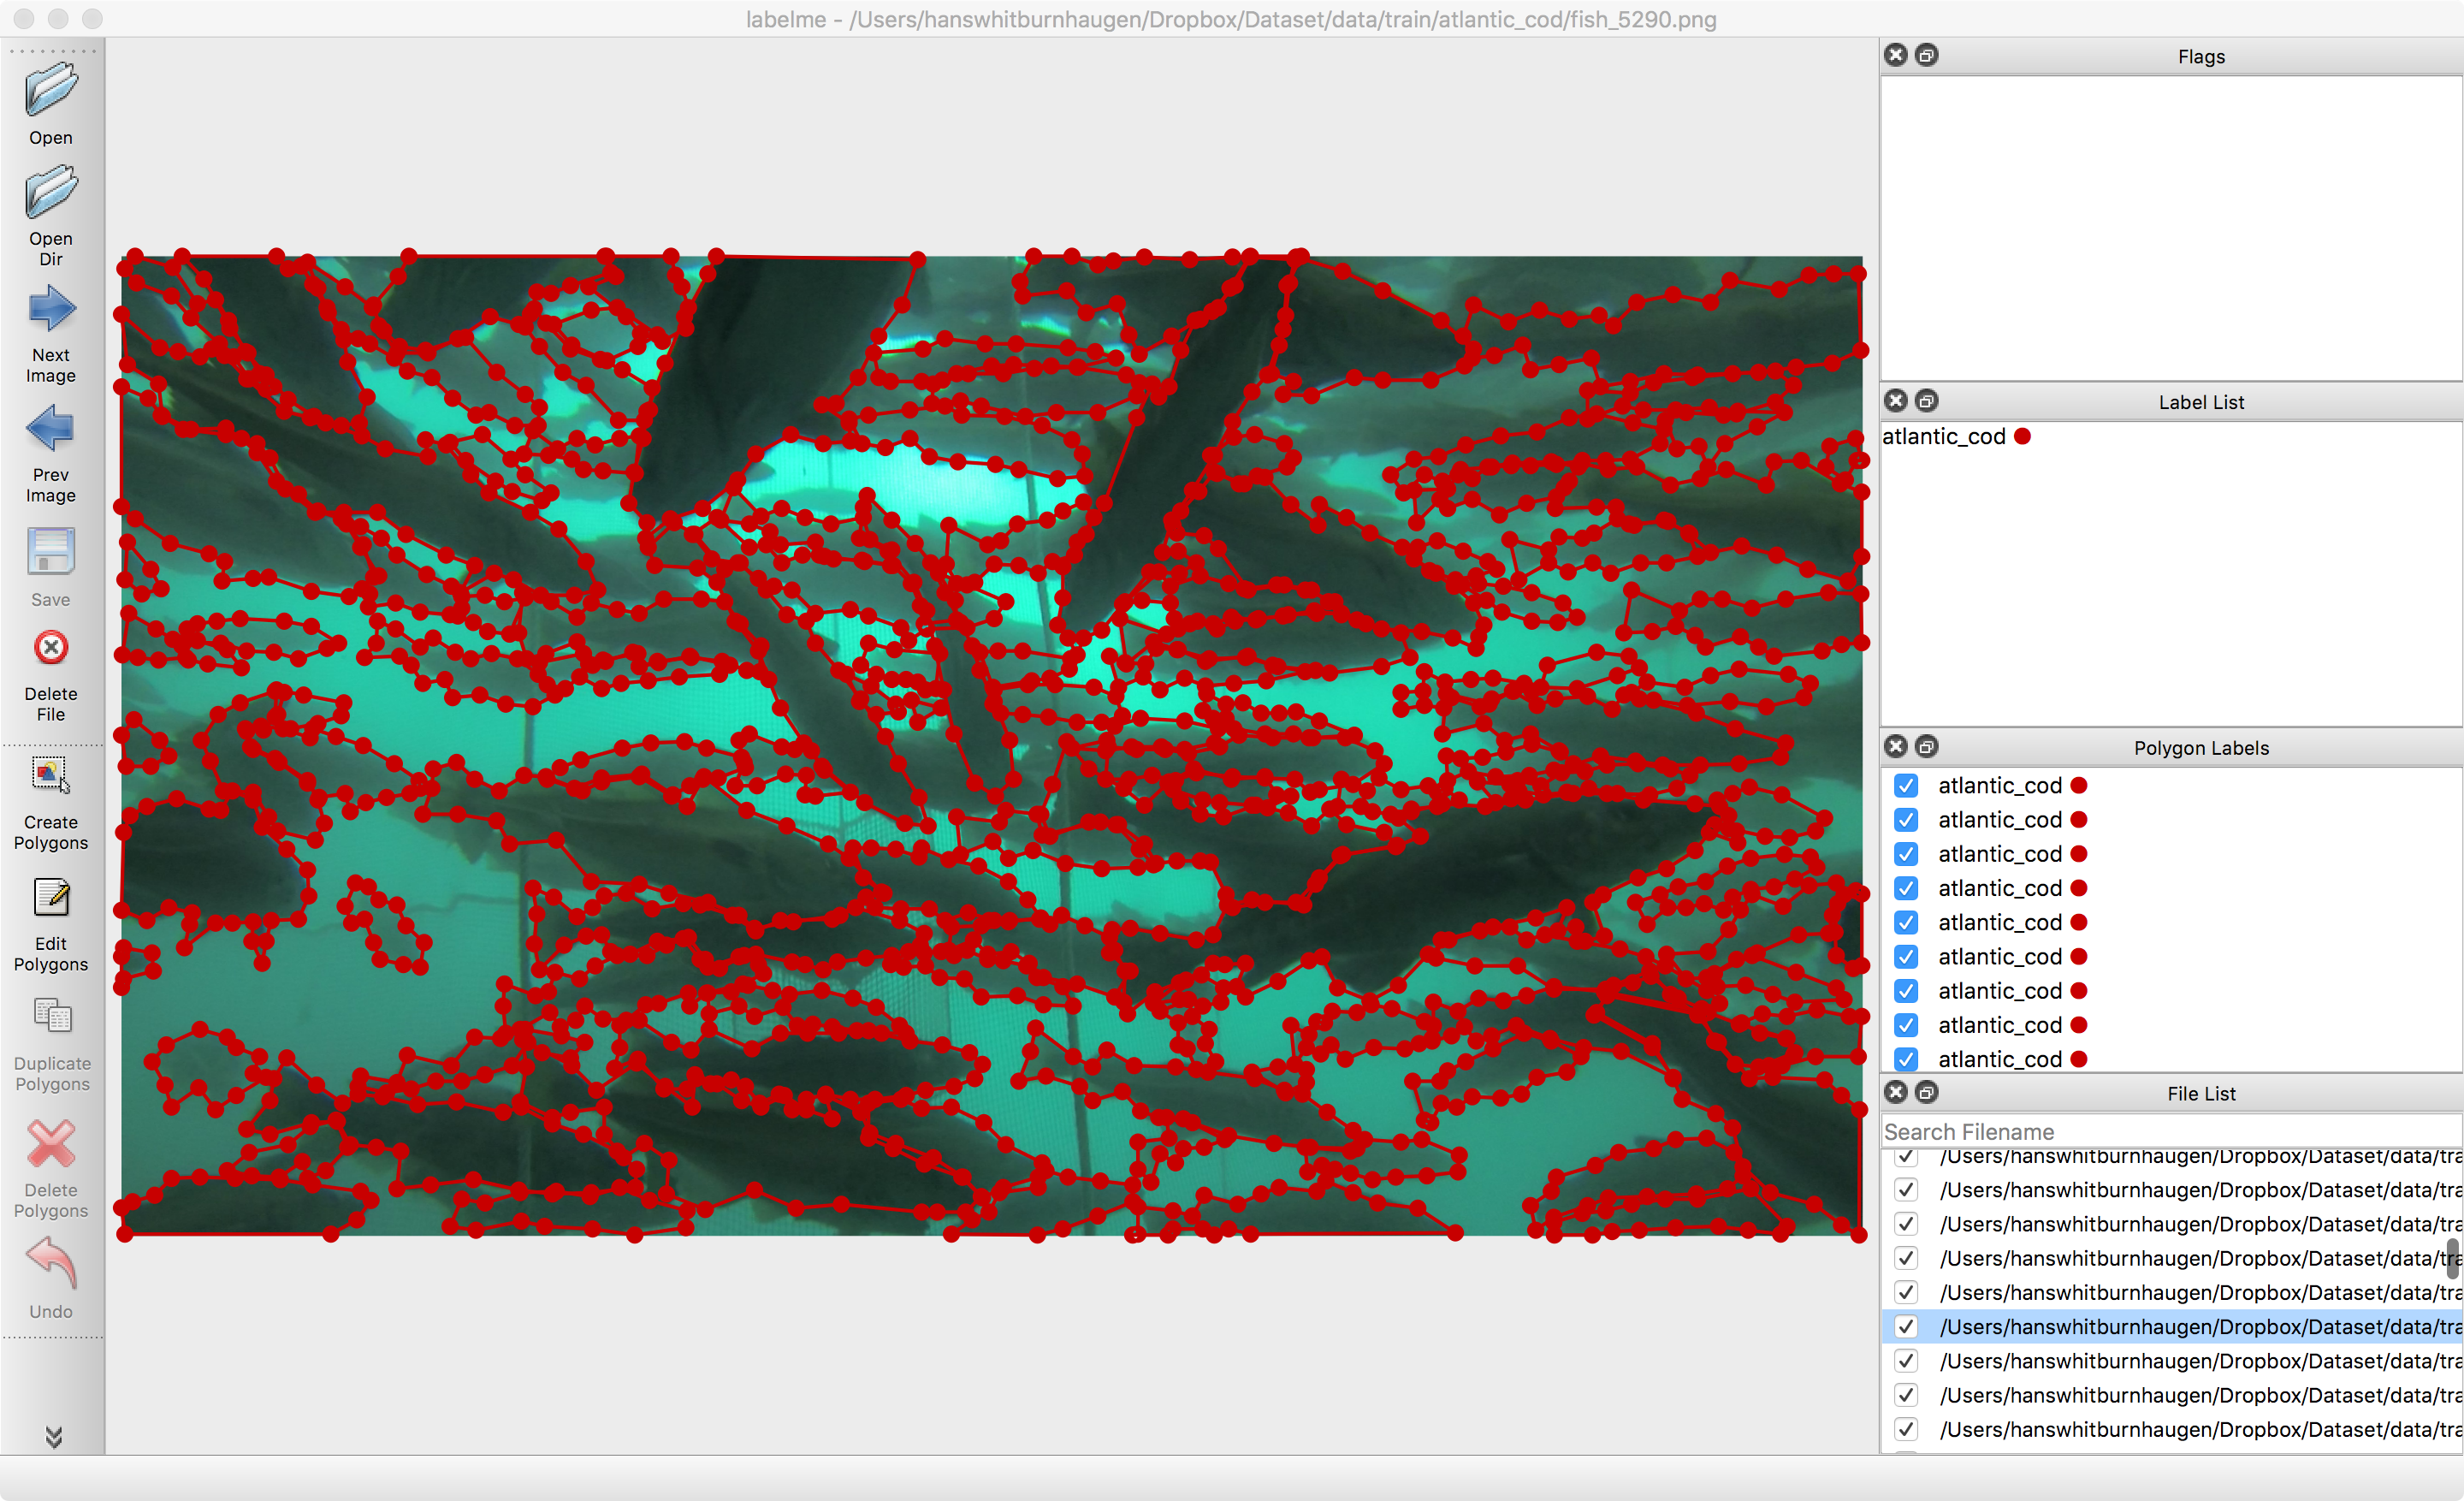
\includegraphics[scale=0.25]{figures/labelme}
\caption{\small \sl Figuren viser dataprogrammet labelme \cite{Wada 2016}. Råbildet er fra en levendelagringsmerd med torsk \cite{Nofima 2020}. \label{fig:labelme}} 
\end{center} 
\end{figure} 
